\let\negmedspace\undefined
\let\negthickspace\undefined
\documentclass[journal]{IEEEtran}
\usepackage[a5paper, margin=10mm, onecolumn]{geometry}
%\usepackage{lmodern} % Ensure lmodern is loaded for pdflatex
\usepackage{tfrupee} % Include tfrupee package

\setlength{\headheight}{1cm} % Set the height of the header box
\setlength{\headsep}{0mm}     % Set the distance between the header box and the top of the text

\usepackage{gvv-book}
\usepackage{gvv}
\usepackage{cite}
\usepackage{amsmath,amssymb,amsfonts,amsthm}
\usepackage{algorithmic}
\usepackage{graphicx}
\usepackage{textcomp}
\usepackage{xcolor}
\usepackage{txfonts}
\usepackage{listings}
\usepackage{enumitem}
\usepackage{mathtools}
\usepackage{gensymb}
\usepackage{comment}
\usepackage[breaklinks=true]{hyperref}
\usepackage{tkz-euclide} 
\usepackage{listings}
% \usepackage{gvv}                                        
\def\inputGnumericTable{}                                 
\usepackage[latin1]{inputenc}                                
\usepackage{color}                                            
\usepackage{array}                                            
\usepackage{longtable}                                       
\usepackage{calc}                                             
\usepackage{multirow}                                         
\usepackage{hhline}                                           
\usepackage{ifthen}                                           
\usepackage{lscape}
\begin{document}

\bibliographystyle{IEEEtran}
\vspace{3cm}

\title{5.2.15}
\author{EE25BTECH11012-BEERAM MADHURI}
% \maketitle
% \newpage
% \bigskip
{\let\newpage\relax\maketitle}

\renewcommand{\thefigure}{\theenumi}
\renewcommand{\thetable}{\theenumi}
\setlength{\intextsep}{10pt} % Space between text and floats


\numberwithin{equation}{enumi}
\numberwithin{figure}{enumi}
\renewcommand{\thetable}{\theenumi}


\textbf{Question}:\\
Solve the system of equations\\
\begin{align*}
    2x + y &=5\\
    3x+2y &=8
\end{align*}
\textbf{Solution:}
The equation of line:
\begin{align}
n^\top x = c
\end{align}
Line L:
\begin{align}
\begin{pmatrix}2 & 1\end{pmatrix}\begin{pmatrix}x \\y\end{pmatrix}= 5
\end{align}

Line K:
\begin{align}
\begin{pmatrix}3 & 2\end{pmatrix}\begin{pmatrix}x \\y\end{pmatrix}= 8
\end{align}
Writing in matrix form:
\begin{align}
\begin{pmatrix}2 & 1 \\3 & 2\end{pmatrix}\begin{pmatrix}x \\y\end{pmatrix}=\begin{pmatrix}5 \\8\end{pmatrix}
\end{align}
The following augmented matrix can be solved by gaussian elimination
\begin{align}
\begin{pmatrix}2 & 1 & | & 5 \\3 & 2 & | & 8\end{pmatrix}\xrightarrow{R_2 \to R_2 - \frac{3}{2}R_1}\begin{pmatrix}2 & 1 & | & 5 \\0 & \frac{1}{2} & | & \frac{1}{2}\end{pmatrix}
\end{align}
Since,
\begin{align}
\rank(A) = \rank(A|b) = 2
\end{align}
the system has a unique solution.

from $2^{\text{nd}}$ row,
\begin{align}
y = 1 \Rightarrow x = 2
\end{align}

$\therefore$ Solution of given system of equations is:$\begin{pmatrix}x \\y\end{pmatrix}$= $\begin{pmatrix}2 \\1\end{pmatrix}$

\begin{figure}[H]
    \centering
    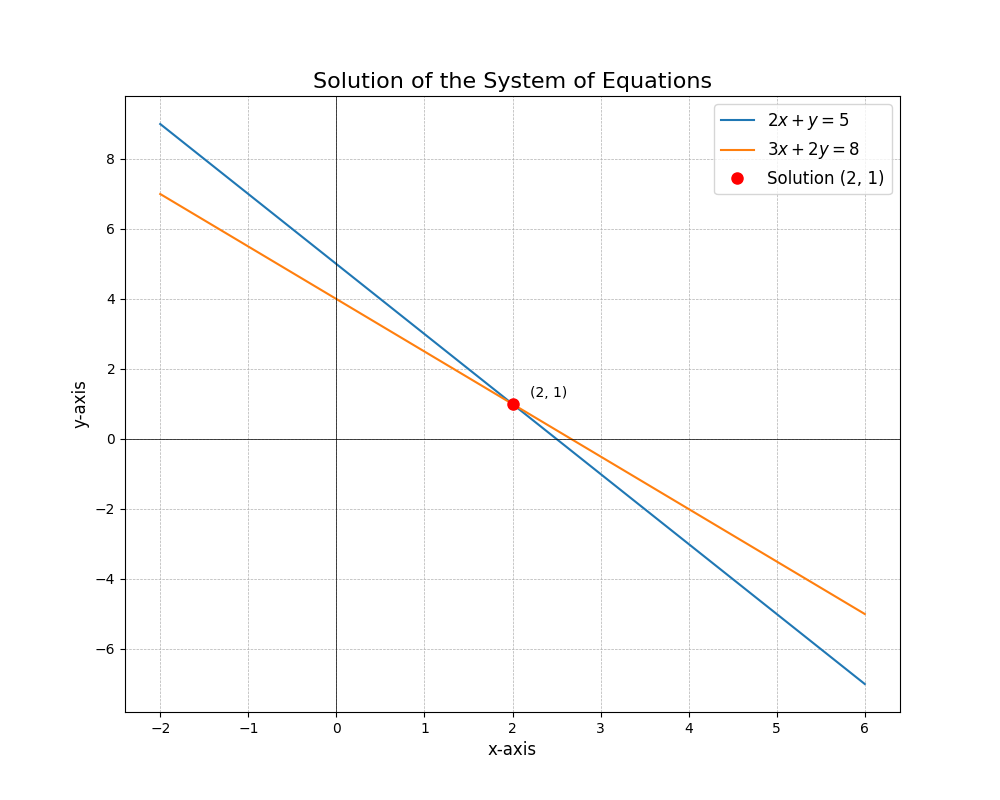
\includegraphics[width=0.85\columnwidth]{figs/graph10.png}
    \caption{5.2.15}
    \label{fig:placeholder}
\end{figure}
\end{document}
